\chapter{Projektmanagement}
\label{pm_cha:Projektmanagement}

\section{Dokumentinfo}

\section{Projektorganisation}
ziele, team (rollen, zuständigkeiten), 
\subsection{Projektziele}
\label{pm_subsec:Projektziele}
Der zentrale Aspekt dieses Projektes war der Wissenserwerb im Bereich Blockchain und die konkrete Anwendung dieses neu erworbenen Wissens durch die Konzeption und Implementation eines IoT Demonstrators. Dieser sollte durch sorgfältige und gründliche Arbeit dem Auftraggeber in einem eigenständig verwendbaren Zustand übergeben werden können. Die konkrete Aufgabenstellung für den Demonstrator wurde ebenfalls im Rahmen dieses Projektes vom Projektteam entwickelt und mit dem Auftraggeber besprochen.

\subsection{Rollen \& Zuständigkeiten}

\begin{table}[H]
\centering
\caption{Projektrollen}
\label{tbl:Projektrollen}
\begin{tabular}{@{}L{4cm}R{4cm}R{4cm}}
\toprule
\multicolumn{1}{l}{Name}   & \multicolumn{1}{r}{Rolle}       & \multicolumn{1}{r}{Oranisation} \\ \midrule
Hirzel Dominik        & Projektteam                     & HSLU – I  \\ \midrule
Schmid Andreas        & Projektteam                     & HSLU – I  \\ \midrule
Dr. Weingärtner Tim   & Vizedirektor Forschung\newline{}Betreuer & HSLU – I  \\ \midrule
Prof. Dr. René Hüsler & Direktor Departement I\newline{}Auftraggeber & HSLU – I \\ \midrule
Schmidlin Diego        & Experte                         & Ruag \\\bottomrule
\end{tabular}
\end{table}

\section{Projektführung}
Im diesem Projekte wurden die vier klassischen Phasen aus SoDa\footnote{https://www.hslu.ch/de-ch/informatik/forschung/themen/software-engineering/soda, 2017} übernommen, jedoch wird in diesem Projektmanagementplan eine andere Terminologie für die Phasen verwendet, um die explorative Methodologie dieses Projektes zu betonen.

\subsection{Projektplanung}

\begin{figure}[H]
\centering
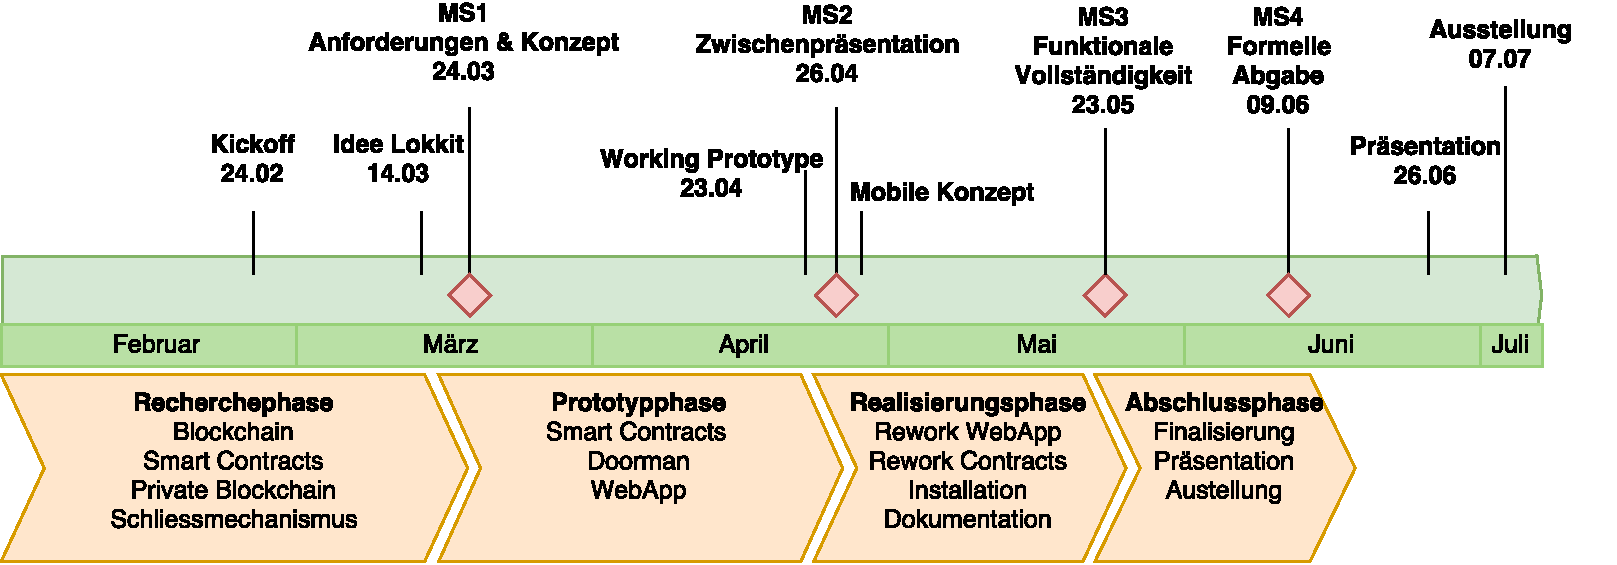
\includegraphics[width=.95\textwidth]{Zeitachse}
\caption{Zeitachse mit Projektphasen und Meilensteine}
\label{fig:Zeitachse mit Projektphasen und Meilensteine}
\end{figure}


\#todo: plan inkl. meilensteine einfügen (aus mid term präsi, evtl updaten)

\paragraph{Initialisierung 24. März}
\label{pm_para:Initialisierung}
Bis am 24. März war die Recherche und Ausarbeitung einer konkreten Aufgabenstellung geplant, die anschliessend implementiert wird. Ein Grobkonzept inklusive Anforderungen für einen Prototyp sollten vorliegen.

Diese Aufgabenstellung wurde am 13. März dem Auftraggeber mitgeteilt und am 14. März besprochen und angenommen (\#todo: siehe email vom 14.3)

\#todo: kommentare des Auftraggebers: siehe Notizen

\#todo: verweis auf requirements für prototyp

\paragraph{Zwischenpräsentation 26. April}
(Prototyp lauffähig) Während er Prototypphase sollte ein definierter Prototyp implementiert werden, der an der Zwischenpräsentation am 26. April vorgeführt werden kann. Dies diente zum einen der raschen Entwicklung einer demonstrierbaren Funktionalität an den Auftraggeber und zum anderen dem Sammeln von konkreten Erfahrungen für das Projektteam im Bereich der Blockchain Technologien. Diese Erfahrungen konnten in der darauf folgenden Phase gewinnbringend eingesetzt und zur Verbesserung der bestehenden Funktionalität verwendet werden.

Der Prototyp mit komplettem Systemdurchstich konnte demonstriert werden. Durch eine Webapp und lokal laufender Ethereum Node wurde demonstriert, dass die Smart Contracts sowie die Anbindung an die private Blockchain funktioniert und auch die Echtzeitkommunikation lauffähig ist.

\paragraph{Formelle Abgabe 9. Juni}
(Dokumentation abgabefertig \& Demonstrator lauffähig) Das Ende des Projektes war der 9. Juni 2017. An diesem Datum sollte der Demonstrator lauffähig, alle Funktionalität dokumentiert und die formellen Testfälle ausgeführt und entsprechend festgehalten sein. 

\#todo: Was hat alles funktioniert, was nicht?

\paragraph{Abschlusspräsentation 26. Juni}
Demonstrator ''gehärtet'' für Abschlusspräsentation und Demonstration (Verbesserungen bei Benutzerfreundlichkeit, Stabilität o.Ä.)
Funktional ist der Demonstrator und jegliche Dokumentation dessen abgeschlossen. Arbeiten, die am Demonstrator nach der Abgabe der Dokumentation gemacht wurden, beschränken sich nur auf den vorführbaren Wert für die Abschlusspräsentation und die Demonstration am 7. Juli.

\#todo: Hier werden wir allfällige weitere Änderungen referenzieren und als v1.1 an der Abschlusspräsi abgeben. Auch Geänderte Dokumente werden als v1.1 abgegeben.

\subsubsection{Recherchephase \emph{Initialisierungsphase}}
\label{pm_subsubsec:Recherchephase}
Im Rahmen des Kick-Off Meetings am 24. Februar übergab der Auftraggeber dem Projektteam den Projektauftrag für einen Demonstrator. Daraufhin wurde ein Rahmenplan erstellt und Meilensteine definiert. In der Recherchephase sollten bestehende Blockchain und IoT Technologien analysiert werden und darauf basierend ein Konzept für einen Demonstrator mit dem Auftraggeber besprochen und definiert werden.

\subsubsection{Prototypphase \emph{Konzeptionsphase}}
\label{pm_subsubsec:Prototypphase}
Das Ziel dieser Phase war es, einen Prototyp zu erstellen, der aufzeigt, dass die Aufgabenstellung so umgesetzt werden kann, wie sie im Konzept definiert wurde. Dabei ist zu beachten, dass das Blockchain Thema im Vordergrund stand. Bei der Umsetzung des Prototyps wurde nach dem explorativen Prinzip gearbeitet, wobei in Intervallen von einer Woche im Projektteam die momentane Situation analysiert und weitere Schritte festgelegt wurden. Hierbei griff das Projektteam sich verändernde Abhängigkeiten (siehe geth 1.6.1\^, status-im, web3 (whisper 5)) auf und versuchte ein limitiertes Set an Anforderungen für den Prototypen zu implementieren, um für die Realisierungsphase eine adäquate zusätzliche Menge Anforderungen definieren zu können.

Am Ende dieser Phase fand die Midterm Präsentation statt, bei der dem Auftraggeber die bisherigen Erfolge, namentlich der Prototyp, vorgeführt wurde. Diese Präsentation diente auch der Besprechung weiterer Anforderungen für die Realisierungsphase, in der der Demonstrator, inklusive der IoT Aspekte, vollumfänglich implementiert werden soll.

\subsubsection{Realisierungsphase}
\label{pm_subsubsec:Realisierungsphase}
Durch die Vorarbeit in den Recherche- und Prototyp- Phasen konnte für die Realisierungsphase eine Menge von Anforderungen definiert werden, die es zu implementieren gilt. Die Vorgehensweise in dieser Phase lehnt sich an das iterativ-inkrementelle Modell von SoDa an, verzichtet jedoch auf explizite Sprints und pflegt keine unterschiedlichen Product- und Sprintbacklogs. Wie auch in der Prototypphase wurden wöchentlich die Arbeiten besprochen und ad-hoc neue Prioritäten für die nächste Woche, basierend auf den noch offenen Anforderungen, definiert. Dies war möglich, da alle Anforderungen bereits in der Recherchephase definiert wurden. Technisch detaillierte User Stories zu definieren war nicht angebracht, da das know-how zur genügenden Fomrulierung solcher grösstenteils während der Realisierung erarbeitet werden musste. Auch die Grösse des Teams und die limitierte Zeitspanne rechtfertigt diese abgespeckte Interpretation von SoDa.

\subsubsection{Projektabschlussphase}
\label{pm_subsubsec:Projektabschlussphase}
In der Projektabschlussphase wurden letzte Integrationstests ausgeführt, um die volle Funktionsfähigkeit des Demonstrators sicherzustellen und allfällige Abweichungen von der Konzeption zu dokumentieren. Weiter wurden die formalen Dokumente vervollständigt und abgeschlossen.

\subsection{Meilensteine}
Am Ende jeder Phase wurde ein Meilenstein mit erwarteten Resultaten definiert.

\subsection{Projektkontrolle}
Der Fortschritt wurde per eMail und in der Midterm Präsentation vom Projektteam an den Auftraggeber kommuniziert.

IST vs SOLL zustand und Massnahmen. (fakultativ)
bspw. bei Rückstand im Projektplan o.Ä.


\subsection{Verantwortlichkeiten}
Dominik Hirzel
\begin{itemize}
    \item Smart Contracts
    \item Android App
    \item Dokumentation
\end{itemize}

\noindent 
Andreas Schmid
\begin{itemize}
    \item Blockchain
    \item IoT
    \item Webapp
    \item Doorman
\end{itemize}


\section{Risikomanagement}
Das Risikomanagement wurde basierend auf der gängigen, und auch in SoDa definierten, Matrixmethode. Die horizontale Achse der Matrix entspricht der Auftretenswahrscheinlichkeit des Risikos, die vertikale Achse spiegelt die Schwere der Auswirkung wieder. Eine höhere Zahl bedeutet hierbei häufiger und schlimmer. Befindet sich die Wahrscheinlichkeit oder die Auswirkung eines Risikos im roten Bereich (vgl. \ref{tbl:Risikomatrix_Leer}), muss mindestens eine Mitigationsmassnahe getroffen werden, um die entsprechende Eigenschaft in den gelben Bereich zu verschieben. Bestenfalls würden Risiken durch besagte Massnahmen eliminiert werden.

\begin{table}[]
\centering
\caption{Risikomatrix Leer}
\label{tbl:Risikomatrix_Leer}
\begin{tabular}{@{}ccccccc@{}}
 & 5 & \cellcolor[HTML]{DF8181} & \cellcolor[HTML]{DF8181} & \cellcolor[HTML]{DF8181} & \cellcolor[HTML]{DF8181} & \cellcolor[HTML]{DF8181} \\
 & 4 & \cellcolor[HTML]{FFFA8F} & \cellcolor[HTML]{FFFA8F} & \cellcolor[HTML]{FFFA8F} & \cellcolor[HTML]{DF8181} & \cellcolor[HTML]{DF8181} \\
 & 3 & \cellcolor[HTML]{92D050} & \cellcolor[HTML]{FFFA8F} & \cellcolor[HTML]{FFFA8F} & \cellcolor[HTML]{FFFA8F} & \cellcolor[HTML]{DF8181} \\
 & 2 & \cellcolor[HTML]{92D050} & \cellcolor[HTML]{92D050} & \cellcolor[HTML]{FFFA8F} & \cellcolor[HTML]{FFFA8F} & \cellcolor[HTML]{DF8181} \\
\multirow{-5}{*}{\rotatebox[origin=c]{90}{Auswirkung}} & 1 & \cellcolor[HTML]{92D050} & \cellcolor[HTML]{92D050} & \cellcolor[HTML]{92D050} & \cellcolor[HTML]{FFFA8F} & \cellcolor[HTML]{DF8181} \\
                             &   & 1                        & 2                        & 3                        & 4                        & 5                        \\
                             &   & \multicolumn{5}{c}{Wahrscheinlichkeit}                                                                                              
\end{tabular}
\end{table}

\subsection{Übersicht}
Risiken werden für jede Phase als Übersicht vollumfänglich tabellarisch festgehalten. D.h., dass nicht nur neue Risiken erfasst sondern auch bestehende Risiken neu evaluiert (oder gestrichen) werden. Hierbei wird bewusst gewisse Redundanz zu Gunsten der Vollständigkeit auf einen Blick in Kauf genommen. Die Risiken werden mit einer Nummer und einem Namen zur einfacheren Identifikation versehen. Eine ausführliche Beschreibung der Risiken, eine Begründung für die Kategorisierung, allfällige Mitigationsmassnahmen und Massnahmen bei Eintreffen des Risikos werden anschliessend gelistet, sollte dies benötigt werden. Die Risiken werden in der Matrix vor und nach der Mitigationsmassnhamen dargestellt. Dabei ist die betonte Zahl (bspw. \emph{1}) die Kategorisierung des Risikos vor und die voll schwarze Zahl (bspw. 1) dieselbe nach den Mitigationsmassnahmen. Sollte keine Massnahmen getroffen worden sein, wird die kursive Zahl ausgelassen. 

\subsection{Risiken Recherchephase}
Während der Recherchephase waren die hauptsächlichen Risiken, dass der frühe Entwicklungsstand aller Blockchain Implementationen nicht die volle Funktionalität bietet, die für einen adäquaten Demonstrator benötigt wird.

\begin{table}[H]
\centering
\caption{Risiken Recherchephase}
\label{tbl:Risiken_Recherche}
\begin{tabular}{lL{8cm}lll}
\toprule
Nr. & Risiko & A & W & Status \\ \midrule
1  & Keine Blockchain Implementation unterstützt Funktionalität für den Demonstrator & 5 & 3 & Neu \\\midrule
2  & Höhere Belastung des Projektteams durch Berufstätigkeit & 2 & 2 & Neu    \\\midrule
\end{tabular}
\end{table}

\begin{table}[H]
\centering
\caption{Risikomatrix Recherche}
\label{tbl:Risikomatrix_Recherche}
\begin{tabular}{@{}ccccccc@{}}
 & 5 & \cellcolor[HTML]{DF8181} & \cellcolor[HTML]{DF8181} & \cellcolor[HTML]{DF8181}1 & \cellcolor[HTML]{DF8181} & \cellcolor[HTML]{DF8181} \\
 & 4 & \cellcolor[HTML]{FFFA8F} & \cellcolor[HTML]{FFFA8F} & \cellcolor[HTML]{FFFA8F} & \cellcolor[HTML]{DF8181} & \cellcolor[HTML]{DF8181} \\
 & 3 & \cellcolor[HTML]{92D050} & \cellcolor[HTML]{FFFA8F} & \cellcolor[HTML]{FFFA8F} & \cellcolor[HTML]{FFFA8F} & \cellcolor[HTML]{DF8181} \\
 & 2 & \cellcolor[HTML]{92D050} & \cellcolor[HTML]{92D050}2 & \cellcolor[HTML]{FFFA8F} & \cellcolor[HTML]{FFFA8F} & \cellcolor[HTML]{DF8181} \\
\multirow{-5}{*}{\rotatebox[origin=c]{90}{Auswirkung}} & 1 & \cellcolor[HTML]{92D050} & \cellcolor[HTML]{92D050} & \cellcolor[HTML]{92D050} & \cellcolor[HTML]{FFFA8F} & \cellcolor[HTML]{DF8181} \\
                             &   & 1                        & 2                        & 3                        & 4                        & 5                        \\
                             &   & \multicolumn{5}{c}{Wahrscheinlichkeit}                                                                                              
\end{tabular}
\end{table}

\paragraph{Risiko 1}
Sollte eine angedachte Funktionalität von keiner Blockchain Implementation unterstützt werden, kann der Demonstrator nicht wie geplant implementiert werden.
\subparagraph{Mitigation}
Präventierende Massnahmen können hier nicht getroffen werden, da die Anforderungen während der Recherchephase basierend auf zur Verfügung stehender Technologie gemacht werden.
\subparagraph{Sofortmassnahmen}
Sollte aufgrund mangelnder Funktionalität der Blockchain Implementationen ein Demonstrator nicht mit angebrachter Funktionalität spezifizierbar sein, werden die Anforderungen an den Demonstrator vereinfacht. Ebenfalls wird mit dem Auftraggeber und Betreuer Kontakt aufgenommen, um die Limitationen in der selbst definierten Aufgabenstellung zu kommunizieren und Alternativen dazu zu suchen.

\subsection{Risiken Prototypphase}
Während der Prototypphase waren die hauptsächlichen Risiken, dass die laufende Entwicklung an \emph{geth} die zu implementierende Funktionalität für den Demonstrator einschränken kann.

\begin{table}[H]
\centering
\caption{Risiken Prototypphase}
\label{tbl:Risiken_Prototyp}
\begin{tabular}{lL{8cm}lll}
\toprule
Nr. & Risiko & A & W & Status \\ \midrule
1  & \sout{Keine Blockchain Implementation unterstützt Funktionalität für den Demonstrator} & 0 & 0 & eliminiert \\\midrule
2  & Höhere Belastung des Projektteams durch Berufstätigkeit & 2 & 2 & erkannt    \\\midrule
3  & Stabilität von geth & 5 & 4 & Neu    \\\midrule
4  & Mangelnde Dokumentation und Hilfestellung zu geth & 4 & 4 & Neu    \\\midrule
\end{tabular}
\end{table}

\begin{table}[H]
\centering
\caption{Risikomatrix Prototypphase}
\label{tbl:Risikomatrix_Prototyp}
\begin{tabular}{@{}ccccccc@{}}
 & 5 & \cellcolor[HTML]{DF8181} & \cellcolor[HTML]{DF8181} & \cellcolor[HTML]{DF8181}\emph{3} & \cellcolor[HTML]{DF8181} & \cellcolor[HTML]{DF8181} \\
 & 4 & \cellcolor[HTML]{FFFA8F} & \cellcolor[HTML]{FFFA8F} & \cellcolor[HTML]{FFFA8F} & \cellcolor[HTML]{DF8181}\emph{4} & \cellcolor[HTML]{DF8181} \\
 & 3 & \cellcolor[HTML]{92D050} & \cellcolor[HTML]{FFFA8F} & \cellcolor[HTML]{FFFA8F}3 & \cellcolor[HTML]{FFFA8F} & \cellcolor[HTML]{DF8181} \\
 & 2 & \cellcolor[HTML]{92D050} & \cellcolor[HTML]{92D050}2 & \cellcolor[HTML]{FFFA8F} & \cellcolor[HTML]{FFFA8F}4 & \cellcolor[HTML]{DF8181} \\
\multirow{-5}{*}{\rotatebox[origin=c]{90}{Auswirkung}} & 1 & \cellcolor[HTML]{92D050} & \cellcolor[HTML]{92D050} & \cellcolor[HTML]{92D050} & \cellcolor[HTML]{FFFA8F} & \cellcolor[HTML]{DF8181} \\
                             &   & 1                        & 2                        & 3                        & 4                        & 5                        \\
                             &   & \multicolumn{5}{c}{Wahrscheinlichkeit}                                                                                              
\end{tabular}
\end{table}

\paragraph{Risiko 1}
Die Implementation geth unterstützt das Ethereum Protokoll, private Netzwerke, Light Nodes (vgl. \ref{para:Light_Node}) (experimentell) und Smart Contracts und kann somit für einen Demonstrator verwendet werden.

\paragraph{Risiko 3}
Da an geth stark entwickelt wird und auch das Ethereum Protokoll Änderungen unterzogen wird, muss damit gerechnet werden, dass die Implementation und auch die Spezifikation geändert werden können. Auch sind kritische Fehler, die die Verwendung von geth oder einzelnen Funktionalitäten verhindern, zu beachten.\cite[EIPs]{github.com/ethereum}
\subparagraph{Mitigation}
Durch ständiges Updaten der Abhängigkeiten kann sichergestellt werden, dass stets eine unterstützte Version des Ethereum Protokolls benutzen wird.
\subparagraph{Sofortmassnahmen}
Das Projektteam integriert sich aktiv in der ethereum Entwicklercommunity durch Teilnahme am gitter chat und Rückmeldung von Fehlern in \emph{geth}.

\paragraph{Risiko 4}
Während der Recherchephase wurde festgestellt, dass die Dokumentation von geth und Teilfunktionen davon nicht immer dem aktuellsten Entwicklungsstand entsprachen. Da an geth stark entwickelt wird und auch das Ethereum Protokoll Änderungen unterzogen wird, muss damit gerechnet werden, dass die Implementation und auch die Spezifikation geändert werden können.
\subparagraph{Mitigation}
Durch ständiges Updaten der Abhängigkeiten kann sichergestellt werden, dass stets eine unterstützte Version des Ethereum Protokolls benutzen wird. Das Projektteam integriert sich auch aktiv in der ethereum Entwicklercommunity durch Teilnahme am gitter chat und Rückmeldung von Fehlern in geht.
\subparagraph{Sofortmassnahmen}
Das Projektteam integriert sich aktiv in der Ethereum Entwicklercommunity durch Teilnahme am gitter chat und Rückmeldung von Fehlern in geth.


\subsection{Risiken Realisierungsphase}
Während der Realisierungsphase waren die hauptsächlichen Risiken, dass die laufende Entwicklung an geth die zu implementierende Funktionalität für den Demonstrator einschränken kann.

\begin{table}[H]
\centering
\caption{Risiken Realisierung}
\label{tbl:Risiken_Realisierung}
\begin{tabular}{lL{8cm}lll}
\toprule
Nr. & Risiko & A & W & Status \\ \midrule
1  & \sout{Keine Blockchain Implementation unterstützt Funktionalität für den Demonstrator} & 0 & 0 & eliminiert \\\midrule
2  & Höhere Belastung des Projektteams durch Berufstätigkeit & 4 & 3 & erkannt    \\\midrule
3  & Stabilität von geth & 5 & 4 & erkannt    \\\midrule
4  & Mangelnde Dokumentation und Hilfestellung zu geth & 4 & 4 & erkannt    \\\midrule
5  & Mangelndes Wissen im Bereich Hardware \& Elektronik & 3 & 3 & neu    \\\midrule
6  & Schliessmechanismen können nicht reverse engineered werden & 5 & 2 & neu    \\\midrule
7  & Einzelteile für den Demonstrator können nicht rechtzeitig geliefert werden & 3 & 4 & neu    \\\midrule
\end{tabular}
\end{table}

\begin{table}[H]
\centering
\caption{Risikomatrix Realisierungphase}
\label{tbl:Risikomatrix_Realisierung}
\begin{tabular}{@{}ccccccc@{}}
 & 5 & \cellcolor[HTML]{DF8181} & \cellcolor[HTML]{DF8181}\emph{6} & \cellcolor[HTML]{DF8181}\emph{3} & \cellcolor[HTML]{DF8181} & \cellcolor[HTML]{DF8181} \\
 & 4 & \cellcolor[HTML]{FFFA8F} & \cellcolor[HTML]{FFFA8F} & \cellcolor[HTML]{FFFA8F}\emph{2},\emph{7} & \cellcolor[HTML]{DF8181}\emph{4} & \cellcolor[HTML]{DF8181} \\
 & 3 & \cellcolor[HTML]{92D050} & \cellcolor[HTML]{FFFA8F} & \cellcolor[HTML]{FFFA8F}3,\emph{5} & \cellcolor[HTML]{FFFA8F} & \cellcolor[HTML]{DF8181} \\
 & 2 & \cellcolor[HTML]{92D050} & \cellcolor[HTML]{92D050}2,5 & \cellcolor[HTML]{FFFA8F} & \cellcolor[HTML]{FFFA8F}4 & \cellcolor[HTML]{DF8181} \\
\multirow{-5}{*}{\rotatebox[origin=c]{90}{Auswirkung}} & 1 & \cellcolor[HTML]{92D050}6 & \cellcolor[HTML]{92D050} & \cellcolor[HTML]{92D050} & \cellcolor[HTML]{FFFA8F} & \cellcolor[HTML]{DF8181} \\
                             &   & 1                        & 2                        & 3                        & 4                        & 5                        \\
                             &   & \multicolumn{5}{c}{Wahrscheinlichkeit}
\end{tabular}
\end{table}

\paragraph{Risiko 2}
Da die Realisierungsphase sehr viel Zeit beansprucht wird dieses Risiko höher bewertet.
\subparagraph{Mitigation}
Alle Beteiligten des Projektteams führen eine transparente Beziehung zu ihrem Arbeitgeber bezüglich ihrem Studium. Die Arbeitgeber unterstützen die Beteiligten des Projektteams in ihrem Studium. Durch frühzeitige Kommunikation mit dem Arbeitgeber bezüglich fixen Terminen oder Projektabschlussphase\footnote{Namentlich der Präsentationterminen, sowie der Intensivwoche anfangs Juni.} wird diesem Risiko entgegengewirkt.
\subparagraph{Sofortmassnahmen}
Rasche Kommunikation mit dem Projektteam und Kompensation der verlorenen Zeit zu einem späteren Zeitpunkt.

\paragraph{Risiko 3}
Auch in der Realisierungsphase wurde weiter stark an geth und dem Ethereum Protokoll entwickelt. Somit muss damit gerechnet werden, dass die Implementation und auch die Spezifikation geändert werden können. Auch sind kritische Fehler, die die Verwendung von geth oder einzelnen Funktionalitäten verhindern, zu beachten.\cite[EIPs]{github.com/ethereum}
\subparagraph{Mitigation}
Durch ständiges Updaten der Abhängigkeiten kann sichergestellt werden, dass stets eine unterstützte Version des Ethereum Protokolls benutzen wird.
\subparagraph{Sofortmassnahmen}
Das Projektteam integriert sich aktiv in der Ethereum Entwicklercommunity durch Teilnahme am gitter chat und Rückmeldung von Fehlern in geht.

\paragraph{Risiko 4}
Während der Recherchephase wurde festgestellt, dass die Dokumentation von geth und Teilfunktionen davon nicht immer dem aktuellsten Entwicklungsstand entsprachen. Da an geth stark entwickelt wird und auch das Ethereum Protokoll Änderungen unterzogen wird, muss damit gerechnet werden, dass die Implementation und auch die Spezifikation geändert werden können.
\subparagraph{Mitigation}
Durch ständiges Updaten der Abhängigkeiten kann sichergestellt werden, dass stets eine unterstützte Version des Ethereum Protokolls benutzen wird. Das Projektteam integriert sich auch aktiv in der ethereum Entwicklercommunity durch Teilnahme am gitter chat und Rückmeldung von Fehlern in geht.
\subparagraph{Sofortmassnahmen}
Das Projektteam integriert sich aktiv in der Ethereum Entwicklercommunity durch Teilnahme am gitter chat und Rückmeldung von Fehlern in geth.

\paragraph{Risiko 5}
Das Projektteam besteht aus Studierenden im Bereich Informatik. Daher kann nicht ausgeschlossen werden, dass für die Implementation des IoT Demonstrators Fachwissen im Bereich Elektronik und Maschinenbau fehlt.
\subparagraph{Mitigation}
Durch vergangene Arbeit in privaten Projekten mit elektronischen Elementen hat das Projektteam begrenzte Erfahrung. Basierend auf diesen bestehenden Kenntnissen kann weiteres Wissen erworben werden. 
\subparagraph{Sofortmassnahmen}
Sollte das benötigte Fachwissen nicht vorhanden sein und nicht in akzeptablem Rahmen aufgebaut werden können, werden Kommilitonen aus den Studienbereich Elektronik und/oder Maschinenbau um Hilfe gebeten, die aus den Fächern PREN1 und PREN2 bekannt sind.

\paragraph{Risiko 6}
Die zur Verfügung gestellten Schliessmechanismen\footnote{Namentlich: Noke und eqiva(vgl. http://www.pearl.de/a-ZX2430-3112.shtml;jsessionid=kCB676D6AFB1D502B2E4B74AA6E98113E)} benutzen teils proprietäre Kommunikationsprotokolle oder sind offiziell nur über ein App ansprechbar.
\subparagraph{Mitigation}
Mit den Herstellern der Schliessmechanismen soll Kontakt aufgenommen werden, um die Wahrscheinlichkeit zu erhöhen, dass diese von lokkit angesprochen werden können. Sollte die Möglichkeit zur Ansprechung der Mechanismen durch Massnahmen des Herstellers erschwert oder verhindert werden, würde der jeweilige Mechanismus zugunsten eines selbst entworfenen Schliessmechanismus nicht weiter verfolgt.
\subparagraph{Sofortmassnahmen}
Da ohnehin ein selbst entworfener Schliessmechanismus eingebaut wird, kann dieser in mehrfacher Ausführung eingebaut werden.

\paragraph{Risiko 7}
Der Demonstrator wird ebenfalls vom Projektteam implementiert. Schliessmechanismen sind unterschiedliche erhältlich, jedoch müssen diese auch mit dem Schliessfachschrank kompatibel sein.
\subparagraph{Mitigation}
Für Teile, deren Lieferfrist einen akzeptable Termin überdauert, sollen Alternativen gesucht werden.
\subparagraph{Sofortmassnahmen}
Da ohnehin ein selbst entworfener Schliessmechanismus eingebaut wird, kann dieser in mehrfacher Ausführung eingebaut werden.


\subsection{Risiken Projektabschlussphase}
In der Projektabschlussphase wird vermehrt ein Augenmerk auf die formellen Dokumente gelegt und somit treffen die meisten technischen Risiken nicht mehr zu.

\begin{table}[H]
\centering
\caption{Risiken Realisierung}
\label{tbl:Risiken_Realisierung}
\begin{tabular}{lL{8cm}lll}
\toprule
Nr. & Risiko & A & W & Status \\ \midrule
1  & \sout{Keine Blockchain Implementation unterstützt Funktionalität für den Demonstrator} & 0 & 0 & eliminiert \\\midrule
2  & Höhere Belastung des Projektteams durch Berufstätigkeit & 4 & 3 & erkannt    \\\midrule
3  & \sout{Stabilität von geth} & 0 & 0 & eliminiert    \\\midrule
4  & \sout{Mangelnde Dokumentation und Hilfestellung zu geth} & 0 & 0 & eliminiert    \\\midrule
5  & \sout{Mangelndes Wissen im Bereich Hardware \& Elektronik} & 0 & 0 & eliminiert    \\\midrule
6  & \sout{Schliessmechanismen können nicht reverse engineered werden} & 0 & 0 & eliminiert    \\\midrule
7  & \sout{Einzelteile für den Demonstrator können nicht rechtzeitig geliefert werden} & 0 & 0 & eliminiert    \\\midrule
\end{tabular}
\end{table}

\begin{table}[H]
\centering
\caption{Risikomatrix Realisierungphase}
\label{tbl:Risikomatrix_Realisierung}
\begin{tabular}{@{}ccccccc@{}}
 & 5 & \cellcolor[HTML]{DF8181} & \cellcolor[HTML]{DF8181} & \cellcolor[HTML]{DF8181} & \cellcolor[HTML]{DF8181} & \cellcolor[HTML]{DF8181} \\
 & 4 & \cellcolor[HTML]{FFFA8F} & \cellcolor[HTML]{FFFA8F} & \cellcolor[HTML]{FFFA8F}\emph{2} & \cellcolor[HTML]{DF8181} & \cellcolor[HTML]{DF8181} \\
 & 3 & \cellcolor[HTML]{92D050} & \cellcolor[HTML]{FFFA8F} & \cellcolor[HTML]{FFFA8F} & \cellcolor[HTML]{FFFA8F} & \cellcolor[HTML]{DF8181} \\
 & 2 & \cellcolor[HTML]{92D050} & \cellcolor[HTML]{92D050}2 & \cellcolor[HTML]{FFFA8F} & \cellcolor[HTML]{FFFA8F} & \cellcolor[HTML]{DF8181} \\
\multirow{-5}{*}{\rotatebox[origin=c]{90}{Auswirkung}} & 1 & \cellcolor[HTML]{92D050} & \cellcolor[HTML]{92D050} & \cellcolor[HTML]{92D050} & \cellcolor[HTML]{FFFA8F} & \cellcolor[HTML]{DF8181} \\
                             &   & 1                        & 2                        & 3                        & 4                        & 5                        \\
                             &   & \multicolumn{5}{c}{Wahrscheinlichkeit}
\end{tabular}
\end{table}

\paragraph{Risiko 3}
Durch Abschluss der Realisierungsphase trifft dies nicht mehr zu.
\paragraph{Risiko 4}
Durch Abschluss der Realisierungsphase trifft dies nicht mehr zu.
\paragraph{Risiko 5}
Durch Abschluss der Realisierungsphase trifft dies nicht mehr zu.
\paragraph{Risiko 6}
Durch Abschluss der Realisierungsphase trifft dies nicht mehr zu.
\paragraph{Risiko 7}
Durch Abschluss der Realisierungsphase trifft dies nicht mehr zu.

\section{Projektunterstützung}
\subsection{Tools}
github, sharelatex, draw.io, inkscape, vim, visual studio code, android studio (full suite), 

\subsection{Konfigurationsmanagement}
\#TODO:Zusammenspiel der Versionen der Komponenten. --> Da nur eine Version veröffentlich wird, ist dies warscheinlich alles V1.0.0.